\documentclass[tikz, border=1cm]{standalone}
\definecolor{darkblue}{RGB}{0,65,125}
\definecolor{lightblue}{RGB}{170,190,225}
\definecolor{darkred}{RGB}{140,30,90}
\definecolor{lightred}{RGB}{220,190,200}
\begin{document}
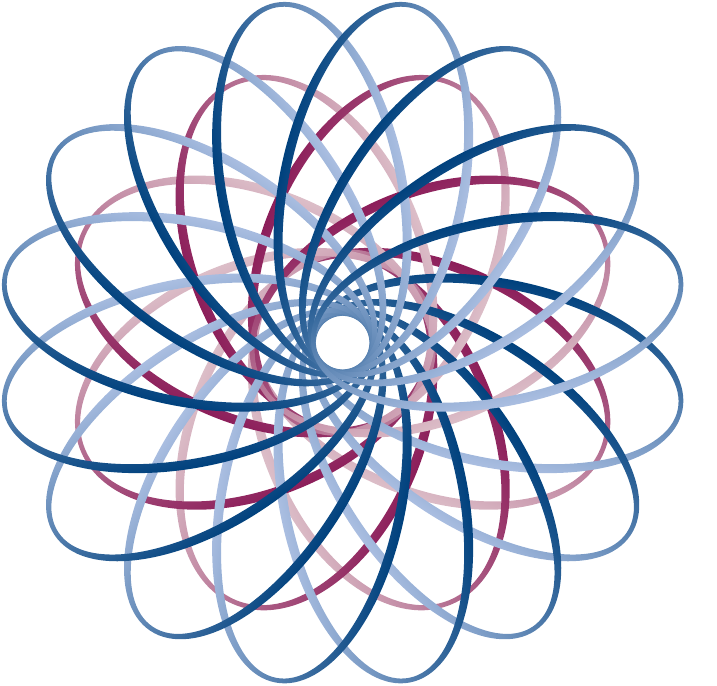
\begin{tikzpicture}

\pgfmathsetmacro{\redN}{8}
\pgfmathsetmacro{\redCradius}{1.2}
\pgfmathsetmacro{\redXradius}{2.4}
\pgfmathsetmacro{\redYradius}{1.5}
\foreach \i in {1,...,\redN}
\shade[top color=darkred, bottom color=lightred, even odd rule, transform canvas={rotate=-(\i-0.5)*360/\redN}] (0:\redXradius-\redCradius) ellipse[x radius=\redXradius, y radius=\redYradius] ellipse[x radius=\redXradius-0.06, y radius=\redYradius-0.12];

\pgfmathsetmacro{\blueN}{16}
\pgfmathsetmacro{\blueCradius}{0.4}
\pgfmathsetmacro{\blueXradius}{2.4}
\pgfmathsetmacro{\blueYradius}{1.2}
\foreach \i in {1,...,\blueN}
\shade[top color=darkblue, bottom color=lightblue, even odd rule, transform canvas={rotate=-(\i-0.5)*360/\blueN}] (0:\blueXradius-\blueCradius) ellipse[x radius=\blueXradius, y radius=\blueYradius] ellipse[x radius=\blueXradius-0.06, y radius=\blueYradius-0.12];

\useasboundingbox (-4,-4) rectangle (4,4);
\end{tikzpicture}
\end{document}